%qqqqqqqqqqqqqqqqqqqqqqqqqqqqqqqqqqqqqqqqqqqqqqqqqqqqqqqqqqqqqqqqqqqqqqqqq
%Quote
\begin{savequote}[50mm]
‘‘The most incomprehensible thing about the universe is that it is 
comprehensible’’
\qauthor{Albert Einstein}
\end{savequote}
%qqqqqqqqqqqqqqqqqqqqqqqqqqqqqqqqqqqqqqqqqqqqqqqqqqqqqqqqqqqqqqqqqqqqqqqqq




%#########################################################################
\chapter{The Cosmological Environment and the Local Group}
\label{cha:Results}


%Reviewed
In this chapter, it is presented the results obtained from the simulations 
des\-cribed in the previous chapter \ref{cha:N-BodySimulations} for the 
dependence of the properties of LG-like systems on the cosmological 
environment in which they are embedded. It is firstly characterized each 
one of the used simulations (CLUES and Bolshoi) with the aim to guarantee 
consistency between the used cosmologies and between the distribution of 
the environmental properties (see section 
\ref{sec:StatisticalPropertiesOfAllSimulations}). After this, in the 
section \ref{sec:PropertiesOfSamplePairs} it is determined the physical
and statistical properties of each one of the defined samples in
\ref{subsec:SampleOfPairsToUse} and it is analysed the correlations 
between the computed properties and the cosmological environment of each 
simulation.



%#########################################################################




%*************************************************************************
%Statistical properties of all simulations
\section{Properties of the Simulations}
\label{sec:StatisticalPropertiesOfAllSimulations}


%Reviewed
One of the first steps for determining the influence of the 
environment on LG-like systems is to construct a \textit{CLG} sample in
unconstrained simulations and thereby obtaining a more robust statistics.
In order to guarantee the consistency of this sample is necessary to 
stablish the equivalence between the distributions of dark matter halos
and analyse the distributions of the cosmological environment of each 
simulation.



	%---------------------------------------------------------------------
	%Halos Properties
	\subsection{Halo Mass Function}
	\label{subsec:Halos_Properties}
	%---------------------------------------------------------------------


%Reviewed
The spatial distribution of the halos exhibits the fine structure of the 
cosmic web, which it is constituted by dark matter. This is exhibited both 
in simulations (see Figure \ref{fig:Halos_Web}) and in cosmological 
observations (see section \ref{sec:CosmologicalObservations}). This 
suggests possible correlations between the properties of the halos and the
environment in which they are embedded, such as it has been demonstrated 
for dark matter halo shapes, the spin parameter and the alignment of 
satellite halos in \cite{libeskind2013}, and for the halo mass 
\cite{lemson1999}. Specially, in the work of \cite{libeskind2013} it is
demonstrated that the V-web classification scheme is more appropriated for
studying correlations with respect to directional properties, like the 
angular momentum of \textit{IP} or \textit{CLG} systems in the section 
\ref{sec:PropertiesOfSamplePairs}.


%Reviewed
\
%.........................................................................
%FOF method in CLUES simulation
\begin{figure}[htbp]
	\centering
	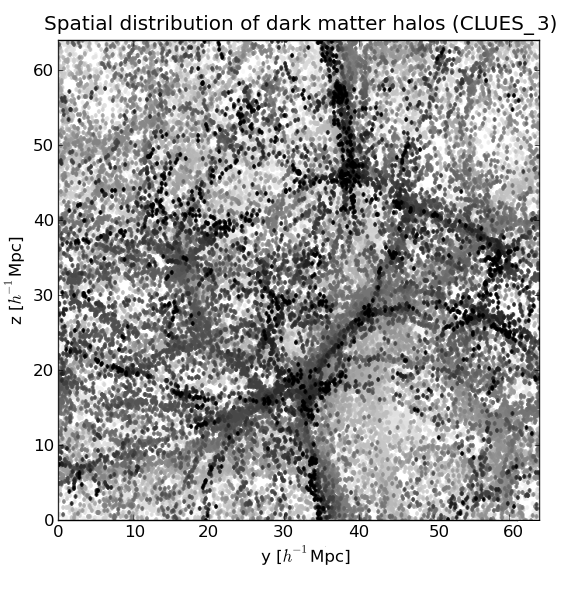
\includegraphics[width=0.58\textwidth]
	{./figures/3_nbody_simulations/Halos_Spatial_Distribution(CLUES_16953).png}

	\caption{\small{Spatial distribution of dark matter halos, exhibiting
	the	characteristic structure of the cosmic web. The colour gradient 
	indicates the depth with respect to the $x$ axis, where black dots 
	are the nearest halos.}}
	
	\label{fig:Halos_Web}
\end{figure}
%.........................................................................


%Reviewed
According to the defining conditions of the \textit{IP} and \textit{CLG} 
samples presented in the subsection \ref{subsec:SampleOfPairsToUse}, the
main property of the halos that is necessary for cons\-tructing these samples
is the halo mass. Therefore it is important to stablish the equivalence 
between the mass distribution of each simulation. The next Figure 
\ref{fig:IMF} shows the results of calculating the cumulative mass 
functions for the Bolshoi simulation and for the three CLUES simulations.


%Reviewed
%.........................................................................
%Integrated Mass Fraction
\begin{figure}[htbp]
	\centering
	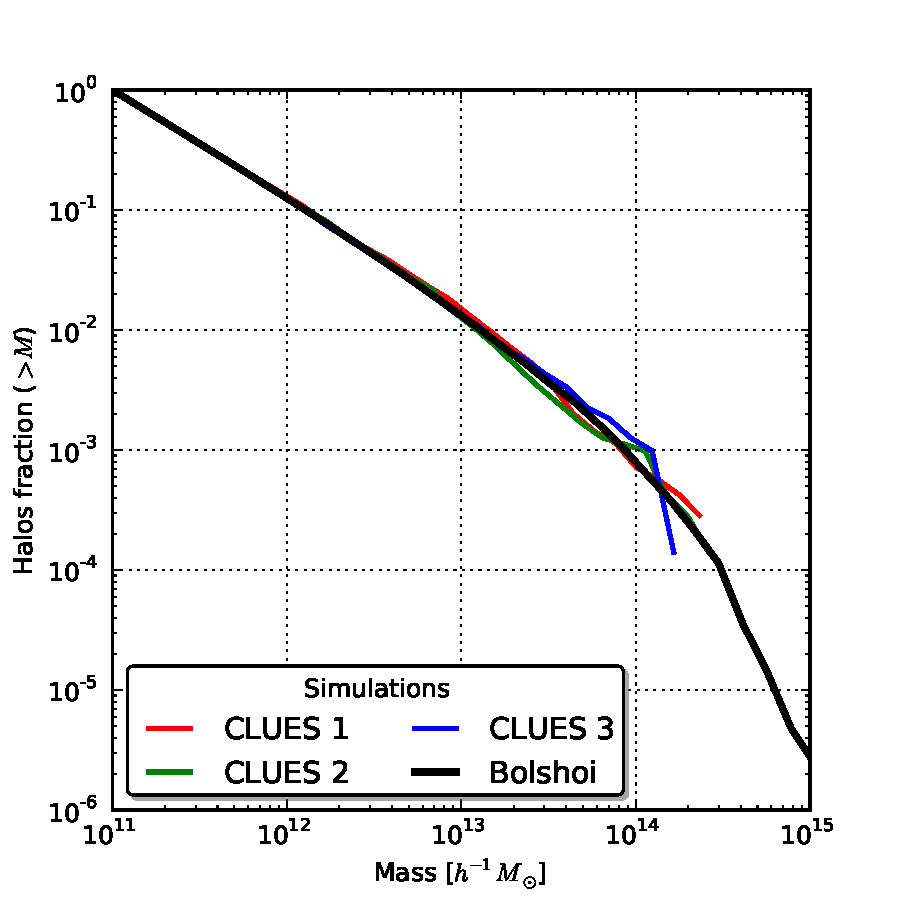
\includegraphics[width=0.70\textwidth]
	{./figures/4_results/Halos_IMF.pdf}
	
	\caption{\small{Cumulative mass functions of the dark matter halos
	(\textit{GH} sample) for each simulation.}}
	\label{fig:IMF}
\end{figure}
%.........................................................................


%Reviewed
For high mass values, the distributions are slightly different due to the 
smaller number of halos in the CLUES simulations, what makes the statistics
less significant in this case. In spite of this, within the mass range 
where the \textit{IH} samples are defined ($5.0 \times 10^{11}\Msun - 
5.0\times 10 ^{12}\Msun$), the distributions are consistent with the 
Press-Schechter mass function formalism \cite{press1974} using the 
cosmological parameters of WMAP7, thereby indicating the equivalence 
between the defined samples for all the used simulations.




	%---------------------------------------------------------------------
	%Environment Properties
	\subsection{Distributions of the Cosmological Environment}
	\label{subsec:Environment_Properties}
	%---------------------------------------------------------------------



%Reviewed
As it has been shown in the section \ref{sec:EnvironmentCharacterization},
the characterization of the cosmological environment is reached by using
physical quantities that indicate the geometric or the dynamical local 
nature of a certain region in the spatial matter distribution. Specially, 
the V-web scheme allows to give account of the dynamics at smaller scales 
of the cosmic web, thereby allowing to characterize and define an adequate 
host environment for halos and other cosmological structures. The next 
Figure shows the results of calculating the distributions for each one of
the eigenvalues of the shear velocity tensor (distributions of 
environment), for both, the cells of the simulations, and the host cells
of the halos of the \textit{GH} sample.


%Reviewed
%.........................................................................
%1D Distribution of Vweb eigenvalues in cells
\begin{figure}[htbp]
	\centering
	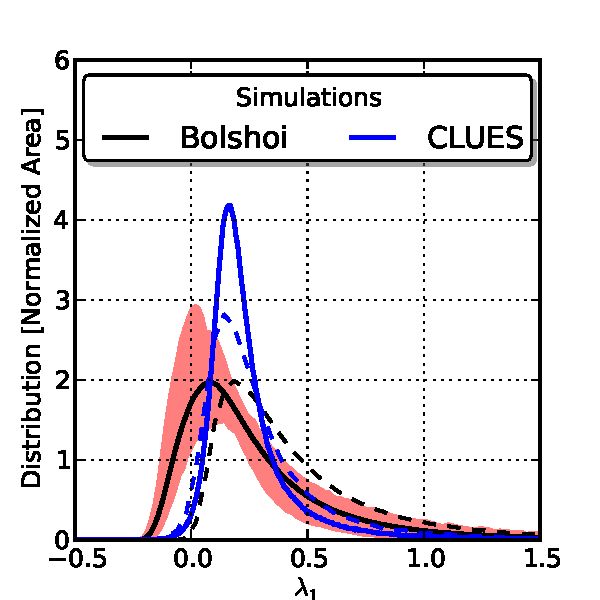
\includegraphics[width=0.38\textwidth]
	{./figures/4_results/Cells_Distro_L1.pdf}
	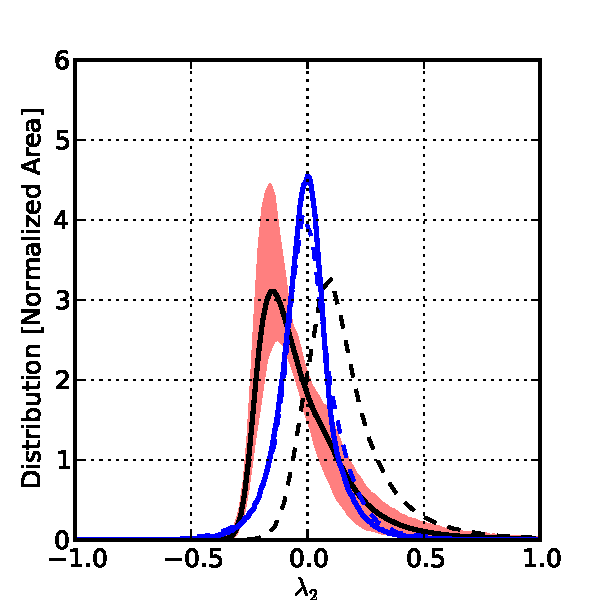
\includegraphics[width=0.38\textwidth]
	{./figures/4_results/Cells_Distro_L2.pdf}
	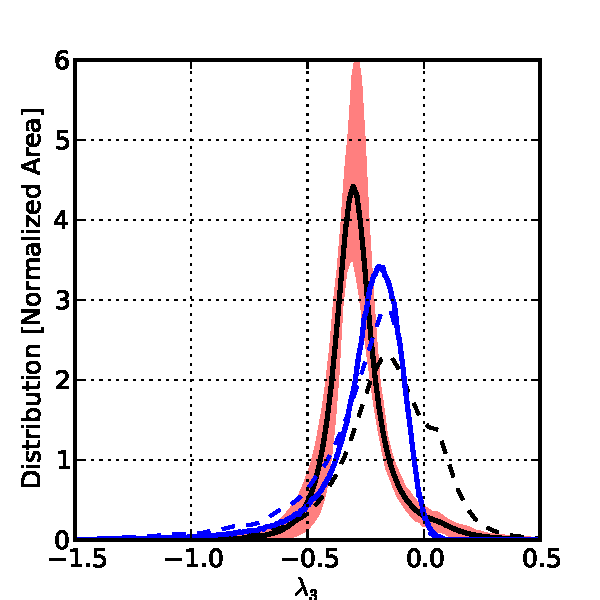
\includegraphics[width=0.38\textwidth]
	{./figures/4_results/Cells_Distro_L3.pdf}

	\caption{\small{ Distributions of eigenvalues of the V-web scheme 
	calculated over all the volume cells (continuous lines) and over the 
	host cells of the dark matter halos defined in the FOF catalogue (dashed 
	lines). All the distributions are normalized such that their area is
	the unity. Resolution of $1.0 h^{-1}$ Mpc/cell and softening parameter
	of one cell size.}}
	\label{fig:1D_Cells_Eigenvalues}
\end{figure}
%.........................................................................


%Reviewed
The main result of the Figure \ref{fig:1D_Cells_Eigenvalues} consists in 
the difference of the distributions for all the volume cells (continuous 
lines) between the Bolshoi simulation and the CLUES simulations \footnote{ 
Because of the high similitude between the distributions of the three 
CLUES simulations, and with the aim of obtaining a more significant 
statistics, they have been merged.}. The effect of the cosmic variance 
(red regions) is included from the calculation of the distributions of 
environment over $64$ sub-volumes of the Bolshoi simulation, with a 
similar size than the CLUES simulations. In spite of this, the 
distributions of environment of the CLUES simulations are outside the 
region of cosmic variance, thereby indicating a different cosmological 
large-scale structure between both simulations.


%Reviewed
A second important result shown by the Figure 
\ref{fig:1D_Cells_Eigenvalues} it is obtained from the distributions of
environment for halos (continuous lines). In the case of Bolshoi, it is
noticed an important bias between the distribution of environment 
associated to the volume cells and the host cells of the halos, thereby 
indicating that the spatial distribution of the halos is not a good tracer
of the large-scale structure of the matter field. This result is 
consistent with the work of \cite{libeskind2013}, where it has been found
an important bias in the distributions of environment according to 
different mass ranges of the halos, also using the Bolshoi simulation. In
the case of the CLUES simulations, the distributions of environment of the
halos are significantly less bia\-sed regarding the volume cells, thus 
indicating for this case that halos do distribute spatially according to
the cosmological environment quantified by using the V-web scheme.


%Reviewed
Finally, in the Figure \ref{fig:Vol_Fraction} it is shown the calculated
mean densities and the vo\-lume fractions for each type of region (see 
section \ref{sec:EnvironmentCharacterization}) according to the threshold
value $\lambda_{th}$. The volume fraction functions are different between
the CLUES and Bolshoi simulations, specially for values close to 
$\lambda_{th} = 0.1$, corresponding to sheet regions. This is due to the 
relative displacement of the peaks of the distributions of environment for
each simulation (see Figure \ref{fig:1D_Cells_Eigenvalues}), what implies
a different behaviour before the criterion to classify the type of region 
from the $\lambda_{th}$ value. In spite of this, the volume fractions are
more or less consistent for both simulations within the range $0.2 \leq 
\lambda_{th} \leq 0.4$ that corresponds to the range where the visual 
impression of the overall density field is better reproduced.


%Reviewed
\newpage
%.........................................................................
%Volume Fraction
\begin{figure}[htbp]
	\centering
	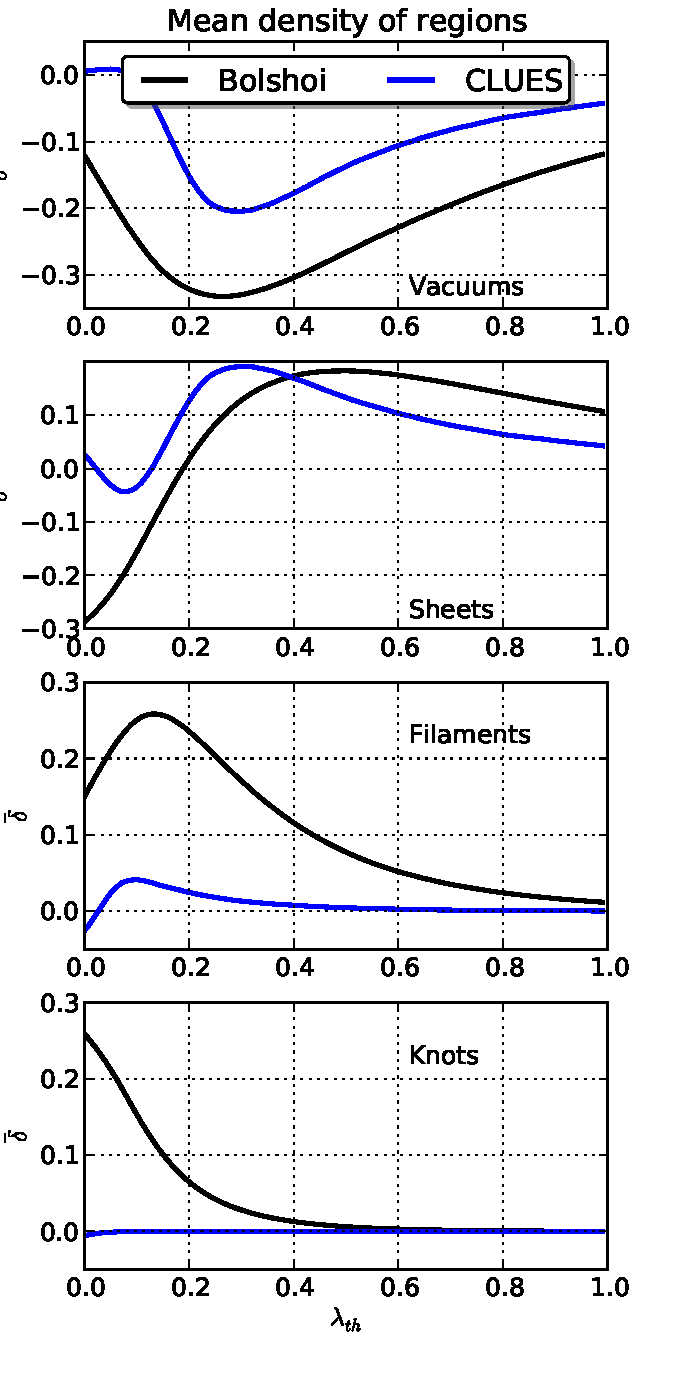
\includegraphics[width=0.43\textwidth]
	{./figures/4_results/Density_Regions.pdf}
	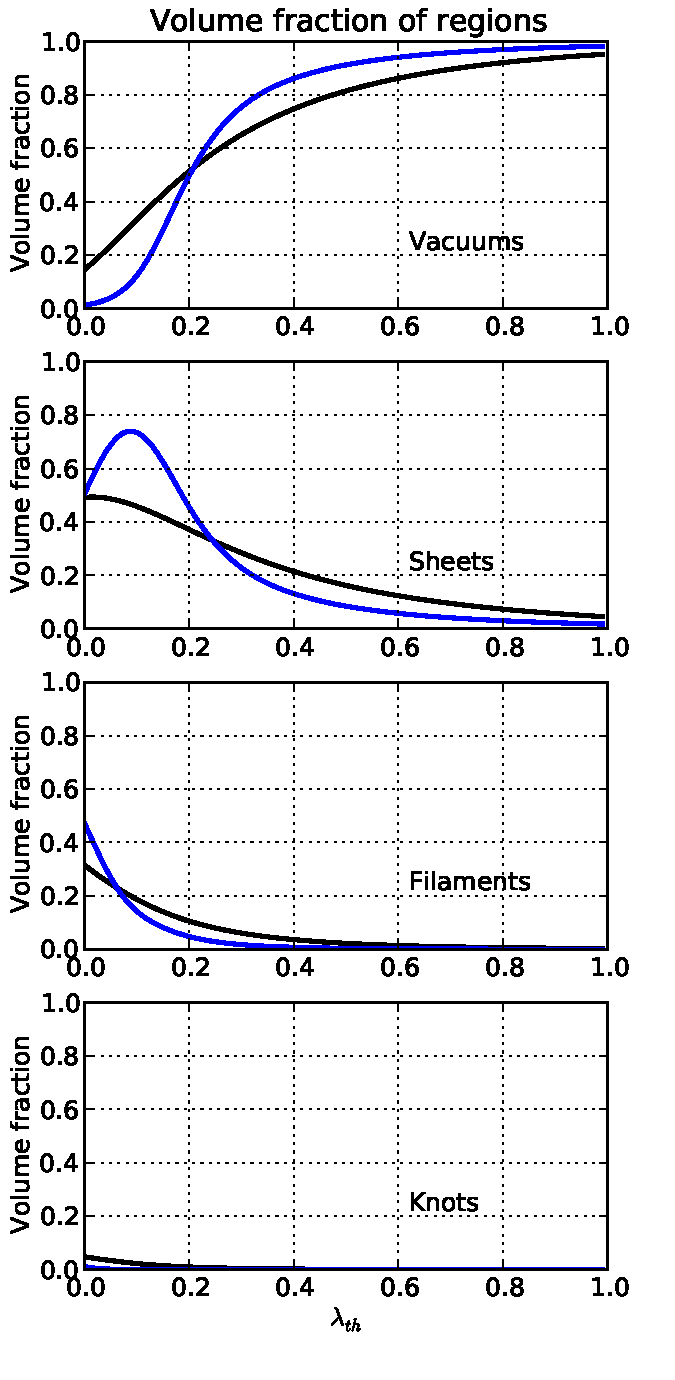
\includegraphics[width=0.43\textwidth]
	{./figures/4_results/Volume_Regions.pdf}
	
	\caption{\small{Mean density parameter for different type of 
	regions in terms of the thre\-shold value $\lambda_{th}$ (left panels).
	Volume fractions normalized for different type of regions, also 
	according to the threshold value $\lambda_{th}$ (right panels).}}
	\label{fig:Vol_Fraction}
\end{figure}
%.........................................................................


%Reviewed
In the figures of the mean density for each type of region, it is shown 
important results regarding the cosmological environment. The first thing
that can be noticed is the difference between the mean densities of both 
simulations for each type of region. For instance for vacuum regions, in
Bolshoi these correspond to regions with a mean density much less than 
the mean density of the entire simulation, whereas in the CLUES 
simulations, the sub-density of vacuum regions is not very pronounced.
Due to the small fraction of knot regions in both simulations (because 
their zero-dimensional geometry), the global structure of the cosmic web
can be understood just in terms of the spatial distribution of vacuums,
sheets and filaments, being filaments the counterpart of vacuums regarding
the density parameter. From this it is expected that the difference 
of the sub-density values of vacuum regions between both simulations 
becomes compensated with a pronounced difference of the over-density 
values of filament regions between both simulations too. The latter has been 
obtained in the same figure, where it can be seen that filament regions of
the Bolshoi simulation are notably denser than filaments in CLUES. In the
case of sheet regions, these correspond to regions with intermediate 
values of density, within a range between filaments and vacuums, therefore
it is expected that the difference of the mean density of these 
regions between both simulation is not very pronounced, such as it can be 
noticed in the same figure.


%Reviewed
%.........................................................................
%Vweb Comparison
\begin{figure}[htbp]
	\begin{center}
	\makebox[\textwidth]{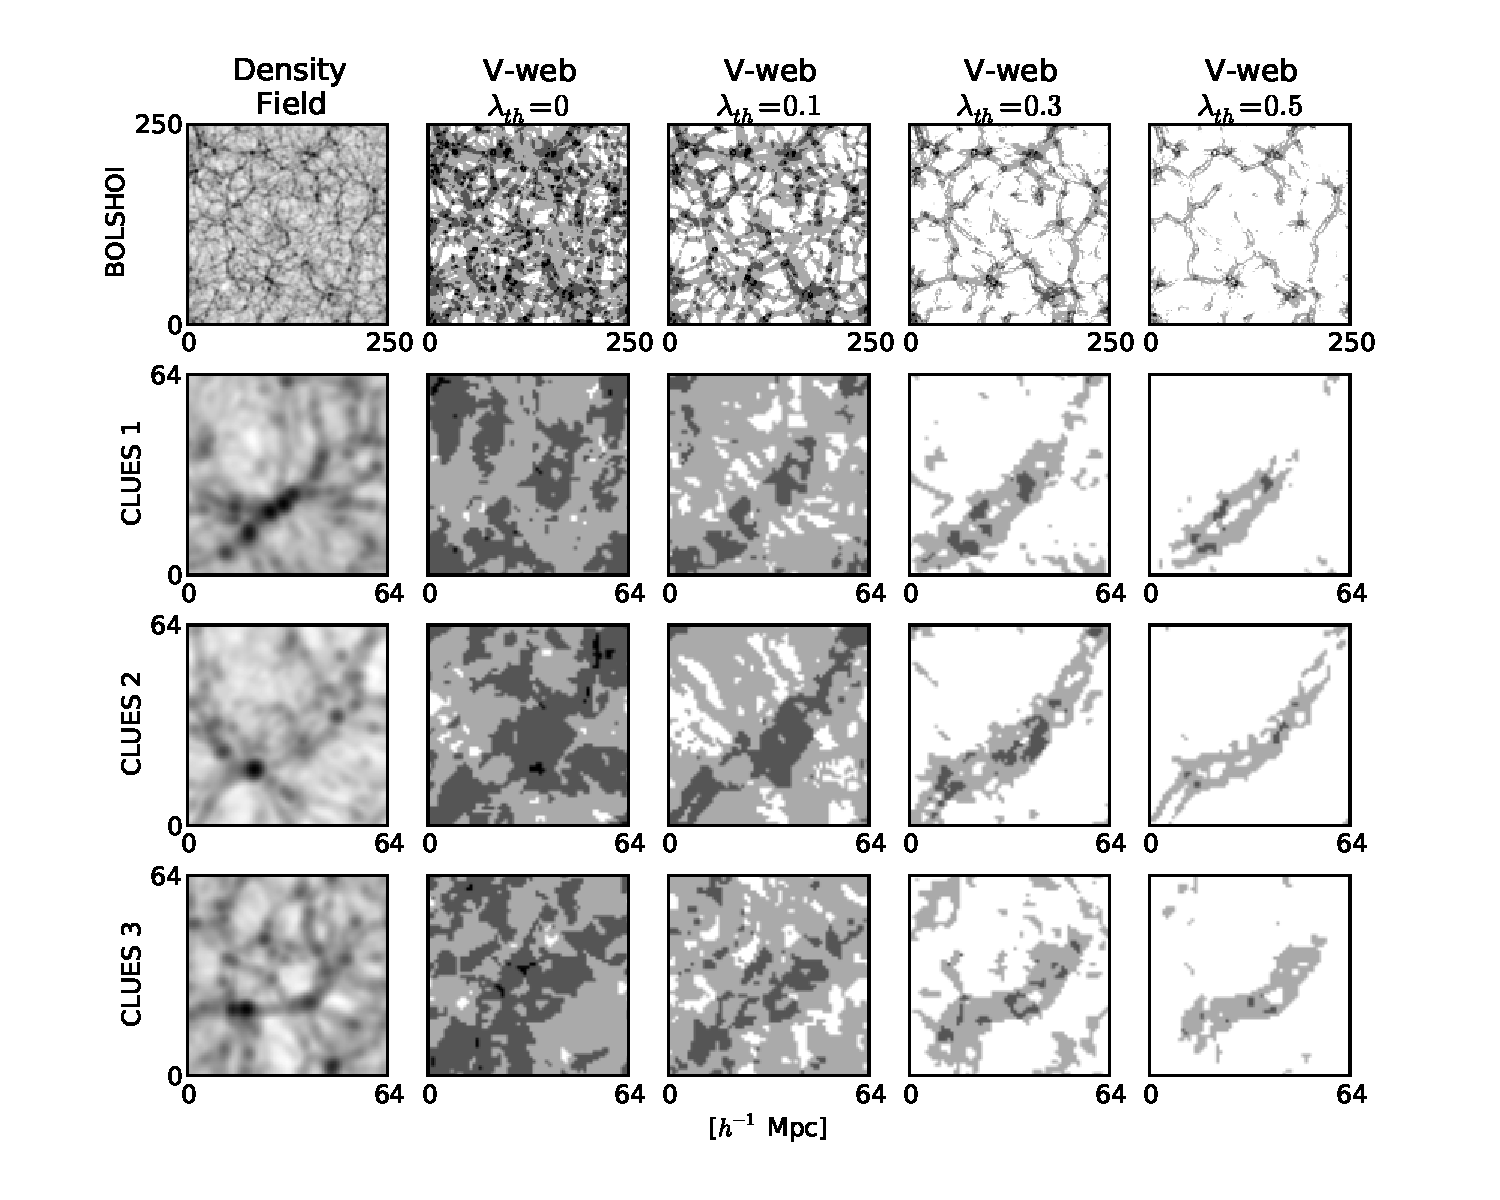
\includegraphics[trim = 10mm 10mm 10mm 9mm, clip,
	width=0.63\paperwidth,angle=0]
	{./figures/4_results/Vweb_Comparison.pdf}}
	\end{center}	
	
	\caption{\small{Comparison between the visual impression obtained by 
	the	V-web scheme for several values of the threshold parameter 
	$\lambda_{th}$. It is used the next classification scheme (Black - Knot,
	Dark gray - Filament, Gray - Sheet, White - Vacuum). The resolution of
	each grid is $1.0 h^{-1}$ Mpc/cell with a Gaussian softening of one cell
	size. The width of each slide is one cell.}}
	\label{fig:Vweb_Comparison}
\end{figure}
%.........................................................................


%Reviewed
The second result shown in the Figure \ref{fig:Vol_Fraction} consists in
determining an optimal threshold parameter $\lambda_{th}$ for reproducing
the visual impression of the cosmic web. As it is shown in this figure,
the volume fractions associated to vacuums and sheets are relatively high
regarding the values of filaments and knots, and this for all the swept 
range of threshold values $\lambda_{th}$. From this it is expected that 
the visual impression of the large-scale matter field is completely 
dominated by the spatial distribution of vacuums and slightly less by 
filaments and sheets. In the case of a low value of the $\lambda_{th}$ 
parameter, e.g. $\lambda_{th}<0.2$, the mean density parameter of sheet 
regions becomes negative, thereby indicating that possibly these regions 
are invading zones that should be catalogued as vacuums, such as it can be 
noticed in the Figure \ref{fig:Vweb_Comparison} for $\lambda_{th} = 0$ o 
$\lambda_{th} = 0.1$. In the case of high values, e.g. $\lambda_{th} > 
0.4\sim 0.5$, the mean density parameter for vacuums is increasing, thus 
indicating that these regions are invading high density zones, which at 
first should be sheets or filaments. This can be noticed in the Figure 
\ref{fig:Vweb_Comparison} for $\lambda_{th} = 0.5$, where all the volume 
is widely dominated by vacuums, thereby loosing the characteristic 
structure of the cosmic web. This analysis suggests that the optimal value
of $\lambda_{th}$ may be that where the mean density of vacuum regions is 
minimized , since this type of region is the most dominant. A result that 
supports this hypothesis is that the found value of $\lambda_{th}$ for 
both simulations is quite similar $\lambda_{th}\approx 0.3$, and 
coincides with the value obtained qualitatively by fitting at first glance 
the visual impression of the cosmological environment.


%Reviewed
To conclude this section, it is discussed the results obtained for the 
distributions of environment. In spite of there is a significant bias 
between the spatial distribution of dark matter halos and the distribution
of the matter field in the Bolshoi simulation, contrary case in the CLUES 
simulations, and there is a marked difference between the mean densities
associated to each type of region for both simulations, the objective of 
constructing a \textit{CLG} sample in the Bolshoi simulation from the 
\textit{LG} systems found in CLUES, as it was mentioned in the chapter 
\ref{cha:N-BodySimulations}, it is to obtain a more faithful sample of 
isolated pairs that also reproduces the same local environment of those
\textit{LG} systems. Then, it is expected that the local dynamic, 
quantifying by the V-web scheme, is independent of the difference between
the distributions mentioned above, retaining the validity of the proposed
construction scheme for the \textit{CLG} sample.



%*************************************************************************




%*************************************************************************
%Properties of sample pairs
\section{Properties of the \textit{CLG} Sample}
\label{sec:PropertiesOfSamplePairs}


%Reviewed
Once it has been determined the consistency between the defined samples 
for both simulations, the next step is to determine their properties. It 
is of special interest to analyse the \textit{CLG} sample in Bolshoi, 
taking as the control sample the \textit{IP} sample, and as the reference 
sample the \textit{LG} sample in CLUES.



	%---------------------------------------------------------------------
	%Determination of their host environment
	\subsection{Determining the Environment}
	\label{subsec:DeterminationOfTheirHostEnvironment}
	%---------------------------------------------------------------------


%Reviewed
As it has been defined in the subsection \ref{subsec:SampleOfPairsToUse} of
the last chapter, the \textit{CLG} sample in the Bolshoi simulation is 
constructed by imposing on the \textit{IP} sample the extra condition of 
reproducing the cosmological environment of the LG-like systems found into 
the CLUES simulations. The main aim of doing this, it is to find a sample 
in the Bolshoi simulation analogous to the \textit{LG} sample, regarding 
their physical properties as well as their abundance. With respect to the 
latter, it is natural to assume, considering the consistency between the 
simulation already determined, that the abundance of a certain sample 
should scale approximately as the volume of the simulation. This fact can
be considered as the first success of the proposed construction scheme, 
since it is reproduced approximately this scale law for the \textit{CLG} 
sample in Bolshoi and the \textit{LG} samples in CLUES (see Table 
\ref{tab:Samples}).


%Reviewed
In spite of the latter, this construction scheme just consists of a cut
in the \textit{IP} sample with respect to the eigenvalues of the shear
velocity tensor of the V-web, evaluated over the host cells of the pair 
systems, which does not imply an adequate reproduction of neither the 
physical properties nor the local cosmological environment of LG-like
systems. For this reason, below it will be analysed possible bias in the 
distributions of environment for the host cells of the \textit{CLG} 
systems.


%Reviewed	
%.........................................................................
%Pathogenic Situation
\begin{figure}[htbp]
	\centering
	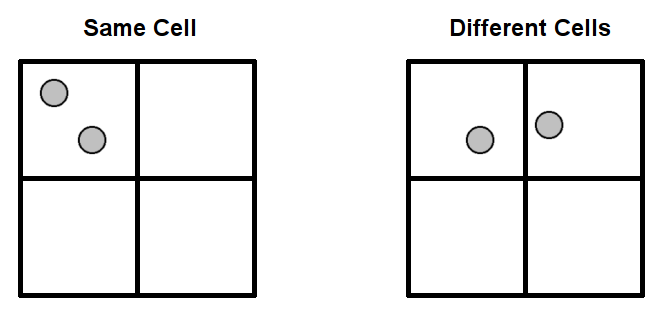
\includegraphics[width=0.5\textwidth]
	{./figures/4_results/Pathogenic_Situation.png}
	
	\caption{\small{Pathological situation regarding the environment of a
	pair system.}}
	\label{fig:Pathogenic_Situation}
\end{figure}
%.........................................................................


%Reviewed
One of the first considerations that should be taken into account for 
quantifying the environment of pair systems (\textit{P}, \textit{IP}, 
\textit{CLG} and \textit{LG} samples), it is that the two halos of the 
pair may be embedded into different cells, such as it is shown in the 
Figure \ref{fig:Pathogenic_Situation}. This pathological situation is 
presented due to the non-point nature of this type of systems and the 
finite resolution of the grid.


%Reviewed
\
%.........................................................................
%Comparison of Lambda in each Halos of Pairs systems
\begin{figure}[htbp]
	\centering
	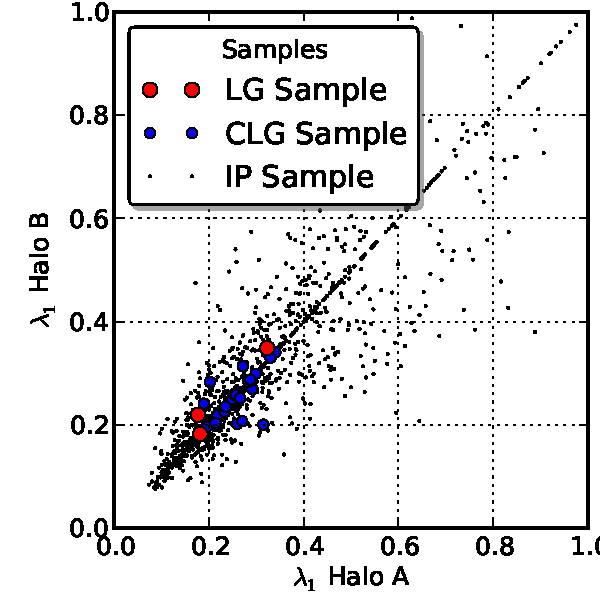
\includegraphics[width=0.46\textwidth]
	{./figures/4_results/CLG_L11_L12.pdf}
	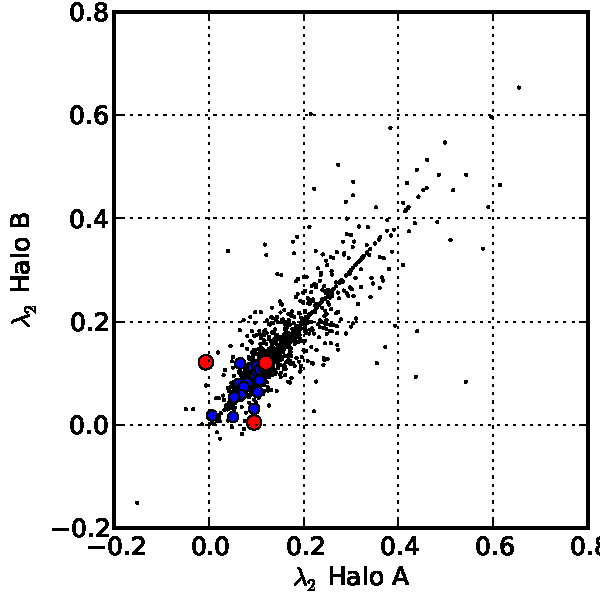
\includegraphics[width=0.46\textwidth]
	{./figures/4_results/CLG_L21_L22.pdf}
	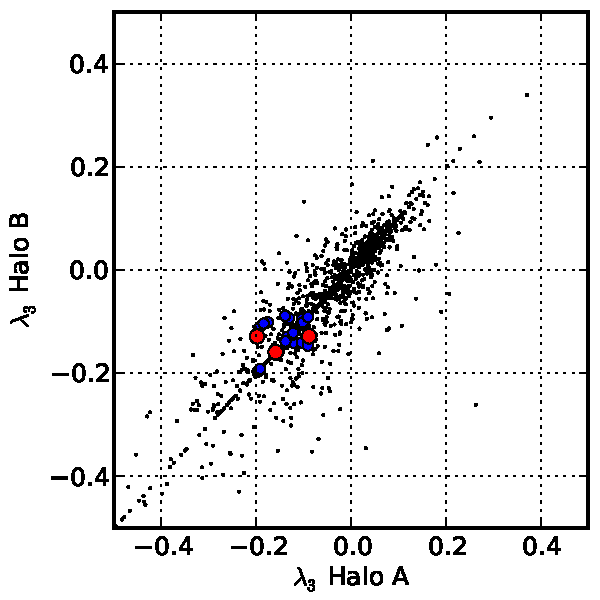
\includegraphics[width=0.46\textwidth]
	{./figures/4_results/CLG_L31_L32.pdf}

	\caption{\small{Comparison between the distributions of the 
	eigenvalues	of the V-web for the two halos of each pair system of
	the \textit{LG}, \textit{CLG} and \textit{IP} samples.}}
	\label{fig:Lambda_Comparison_Pairs}
\end{figure}
%.........................................................................


%Reviewed
In order to quantify this effect, in the Figure 
\ref{fig:Lambda_Comparison_Pairs} are plotted the distributions of each 
eigenvalue of the V-web for each one of the halos in the pair samples. The
ideal situation, where both halos share the same cell, it would correspond
to a straight line with a slope of $45^o$, whereas the pathological 
situations are responsible of the observed dispersion. A way to solve this 
issue is to decrease the resolution of the grid, such that both halos are 
embedded in the same cell, but this would cause a losing of information 
regarding the local environment of the pair system. Due to the Gaussian 
softening of one cell size ($\sim 1 h^{-1}$ Mpc) that has been applied a 
priori over the eigenvalues fields, possible variations between neighbour
cells are neglected, such as it is shown for the most of \textit{IP} 
systems in the figure. Taking into account the latter and the local 
dynamic of pair systems is dominated by the more massive dark halo, by 
convention it will be taken the host cell of this halo as the 
representative of the entire system.


%Reviewed
\
%.........................................................................
%2D Distribution of Vweb eigenvalues in sairs samples
\begin{figure}[htbp]
	\centering
	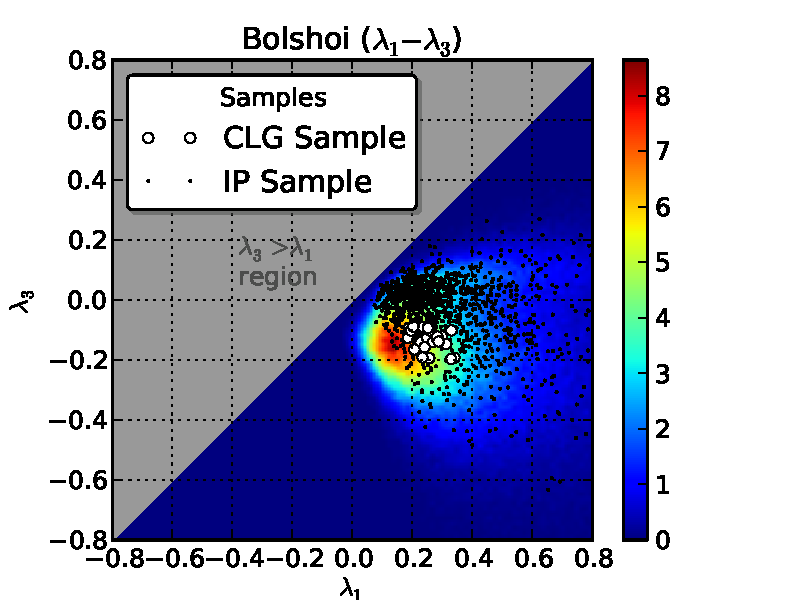
\includegraphics[trim = 0mm 0mm 15mm 0mm, clip, width=0.49\textwidth]
	{./figures/4_results/CLG_Environmet_L1L3.pdf}
	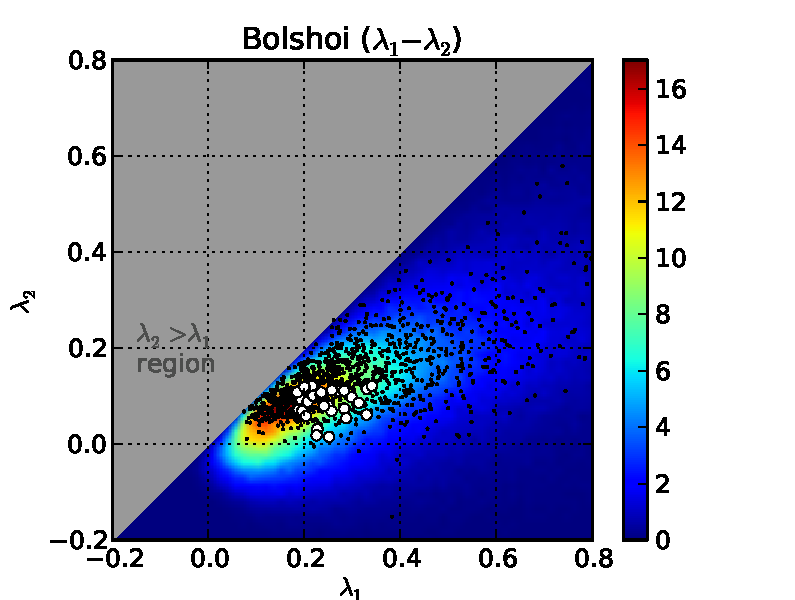
\includegraphics[trim = 0mm 0mm 15mm 0mm, clip, width=0.49\textwidth]
	{./figures/4_results/CLG_Environmet_L1L2.pdf}
	
	\caption{\small{2D distributions of the cosmological environment for
	the defined samples, $\lambda_1$--$\lambda_3$ (left panel) and 
	$\lambda_1$--$\lambda_2$ (right panel). The background histogram, 
	plotted in colours, corresponds to the distribution of environment
	for all the halos in Bolshoi (\textit{GH} sample), its resolution is
	$100\times 100$ for the shown range and it is normalized with respect 
	to its area. The black dots corresponds to the distribution of the 
	\textit{IP} sample and finally the white dots to the \textit{CLG}
	sample.}}
	\label{fig:2D_Samples_Eigenvalues}
\end{figure}
%.........................................................................


%Reviewed
Once it has been determined how to quantify the environment of pair 
systems, in the Figure \ref{fig:2D_Samples_Eigenvalues} is illustrated the
distribution of the samples \textit{GH}, \textit{IP}, \textit{CLG}. As it
has been shown in the subsection \ref{subsec:Environment_Properties}, the
distribution of environment for halos in Bolshoi are considerably biased
with respect to the distribution of the volume cells. In spite of this,
and taking into account that the construction of pair systems it is made
from the sample of halos, it is more interesting to perform comparisons
between the distributions associated to halos (coloured histograms in
the same figure). As it was defined in the subsection 
\ref{subsec:SampleOfPairsToUse}, the \textit{IP} sample is constructed 
such that it is guaranteed its gravitational isolation with respect to
more massive halos and other structures, that is why there are two effects
that compete regarding the distribution of environment of these systems.
In the first effect, it is expected that the abundance of pairs is more
favourable around environments where there are more halos, whereas in the 
second effect, precisely the over-abundance of halos becomes unfavourable
due to the criterion of gravitational isolation. According to the results, 
the second effect is more dominant on the \textit{IP} sample with respect
to all the halos, while for the \textit{P} sample the bias is not longer
presented\footnote{ The latter is not shown in the Figure 
\ref{fig:2D_Samples_Eigenvalues}, but it is easily computed.}
 

%Reviewed
In order to conclude the analysis of the previous figure, it is discussed 
about the distribution of environment for the \textit{CLG} systems in the
Bolshoi simulation. In spite of this distribution is artificially biased 
because of the selection criterion, it is interesting to notice that the
range of the eigenvalues that delimits this sample is relatively reduced, 
thereby indicating that the three LG-like systems in the CLUES simulations
share a similar local dynamic. Although the latter may be an effect 
established a priori by construction due to the constrained nature of the
CLUES simulations, it is still interesting the bias that this feature 
produces on the distribution of environment of the \textit{CLG} sample
regarding all the halos and the \textit{IP} sample.


%Reviewed
To quantify the produced biases in each sample regarding a specific type
of environment (See Figure \ref{fig:ClassificationSchemeTweb}), in the 
next Figure \ref{fig:Samples_Fraction} it is plotted the fractions of 
objects into each type of region. In the optimal range of the threshold 
value $0.2\leq \lambda_{th}\leq 0.4$, defined in the subsection 
\ref{subsec:Environment_Properties}, it is noticed important differences
between each one of the samples, specially for the \textit{CLG}. As it has
been previously mentioned, the effect of the gravitational isolation 
produces a bias between the distribution of environment of the halos 
\textit{GH} and the distribution of the \textit{IP} systems. This can be 
clearly noticed for each one of the number fractions in the optimal range 
of $\lambda_{th}$. In the case of vacuums, the dominant fraction is that 
associated to \textit{IP}, but in the case of sheet regions, the fraction
of both samples are comparable, and even more, in the filament and knot 
regions, the dominant fractions is that corresponding to halos \textit{GH}.
This indicates that \textit{IP} systems are more abundant in regions of 
low to middle density of halos, but even so, there are still a 
considerable fraction within sheet and filament regions, so it is not 
possible to associate a specific type of region to these systems. Finally,
the \textit{CLG} systems present an important bias compared with the two
previously discussed samples, being specially interesting that produces
regarding the \textit{IP} sample, due to the \textit{CLG} sample is a 
sub-sample of this. Again, taking into account the optimal range of
$\lambda_{th}$, it is possible, in this case, to associate a certain type
of region to the \textit{CLG} sample, being these systems preferentially
in sheet and vacuum regions.


%Reviewed
\
%.........................................................................
%Number Fraction of each sample in differents type of regions
\begin{figure}[htbp]
	\centering
	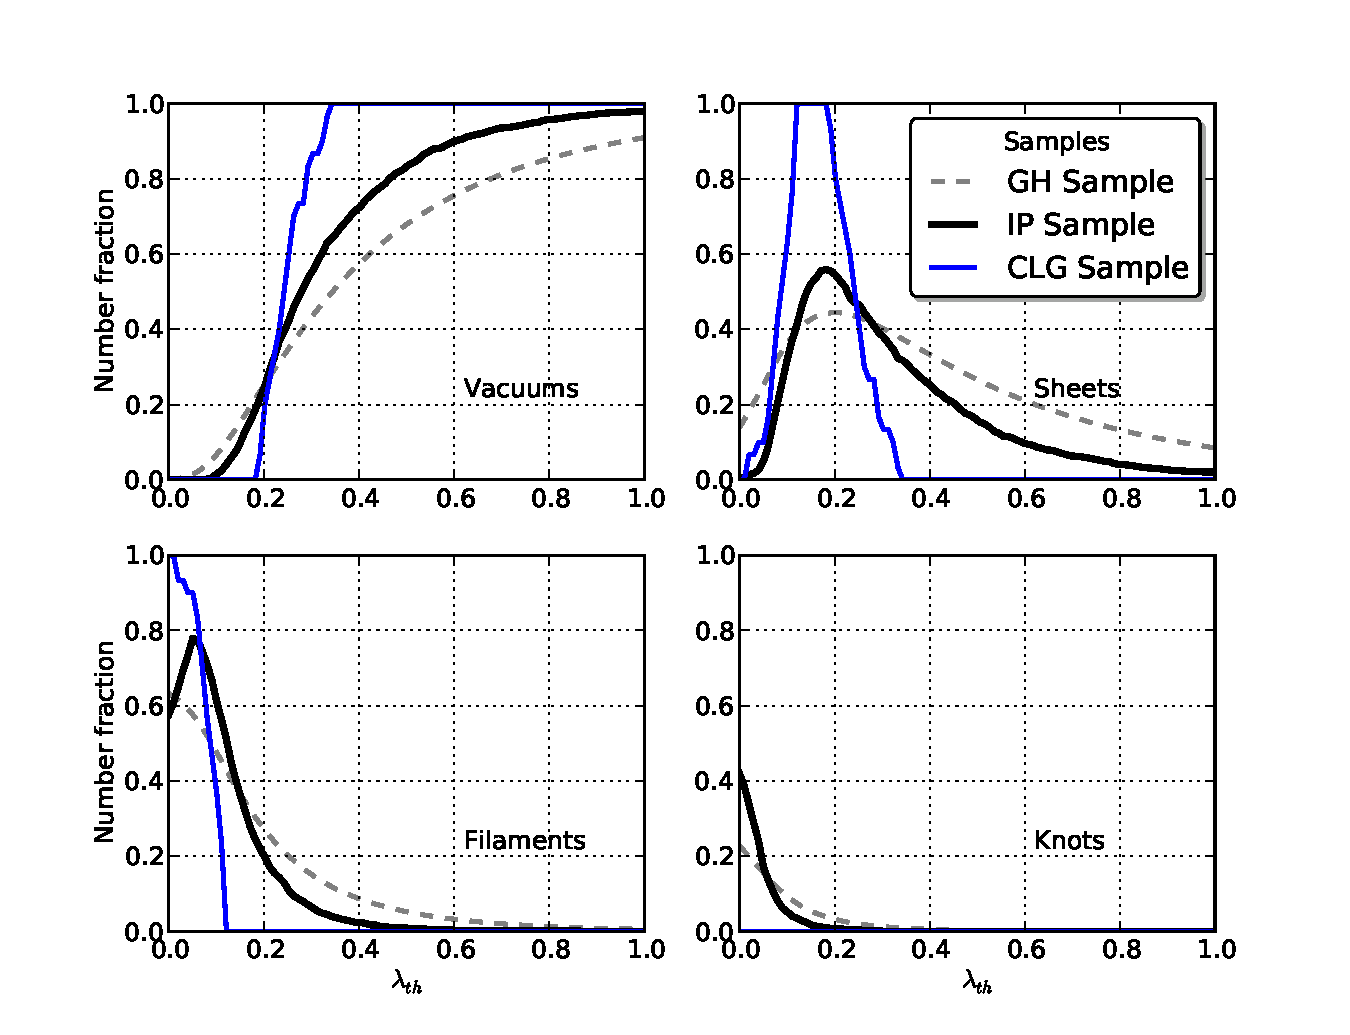
\includegraphics[trim = 8mm 5mm 12mm 12mm, clip, width=0.85\textwidth]
	{./figures/4_results/CLG_Classification_Env.pdf}
	
	\caption{\small{Object fractions in different regions in terms of the
	threshold value $\lambda_{th}$. In the case of the \textit{GH} sample,
	it is counted the number of halos, whereas for the \textit{IP} and 
	\textit{CLG} samples it is counted the number of pair systems.}}
	\label{fig:Samples_Fraction}
\end{figure}
%.........................................................................


%Reviewed
In spite of the classification scheme used, the above conclusions depend
on the selected $\lambda_{th}$ parameter, and although it has been 
reasonably bounded in an optimal region where it is reproduced de visual
impression, it is still a free parameter. In order to solve this, it is 
introduced the fractional of anisotropy (FA) with the normalization used
in \cite{libeskind2013}


%.........................................................................
%Fractional Anisotropy
\eq{eq:FA}
{ FA = \frac{1}{\sqrt{3}}\sqrt{ \frac{ (\lambda_1 - \lambda_3)^2 + 
(\lambda_2 - \lambda_3)^2 + (\lambda_1 - \lambda_2)^2}{ \lambda_1^2 + 
\lambda_2^2 + \lambda_3^2} } }
%.........................................................................


%Reviewed
This quantity allows to quantify the anisotropy degree of the local cosmic
environment, being $FA=1$ a highly anisotropic region, whereas $F=0$ is 
instead a highly isotropic region. Furthermore this quantity is independent
of any free parameter chosen a priori. According to the result obtained by
\cite{libeskind2013}, regions of low isotropy would correspond to knots 
due to their characteristic isotropic collapse, while regions of high 
isotropy would correspond to vacuums due to their non-uniform expansion. 
In the case of filament and sheet regions, the fractional anisotropy is 
extendedly distributed over middle values, thus indicating that the 
dynamic of these type of regions is more complex. Even so, there is a 
slight tendency towards low values in the case of filaments and high 
values for sheets.


%Reviewed
%.........................................................................
%Anisotropy Fractional for pairs samples
\begin{figure}[htbp]
	\centering
	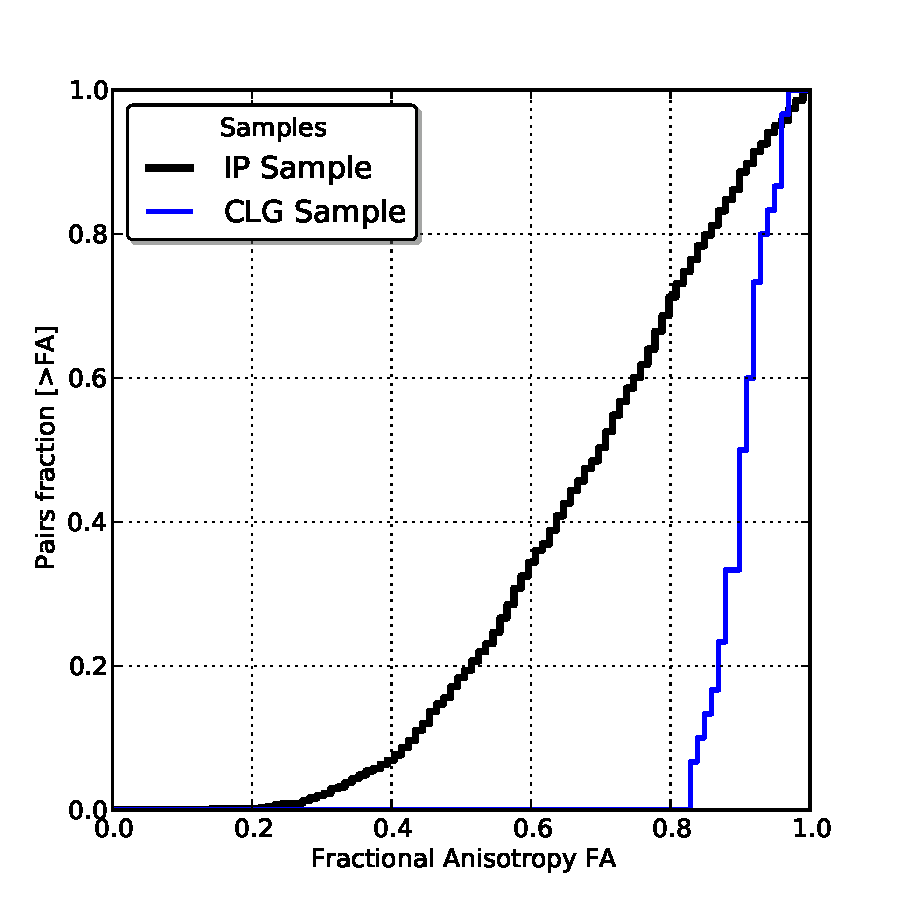
\includegraphics[trim = 0mm 0mm 0mm 10mm, clip, width=0.8\textwidth]
	{./figures/4_results/CLG_FA_Hist.pdf}
	
	\caption{\small{Integrated histogram of the fractional anisotropy for
	the \textit{IP} and \textit{CLG} samples.}}
	\label{fig:FA_samples}
\end{figure}
%.........................................................................	


%Reviewed
In the Figure \ref{fig:FA_samples}, it is calculated the integrated 
histograms of the fractional anisotropy for the \textit{IP} and 
\textit{CLG} samples. The first result is associated to the distribution
of \textit{IP} systems, which is highly homogeneous for middle values
(approximately $0.4 < FA < 0.9$) as it is evidenced by the constant slope
in the histogram. This implies that \textit{IP} systems are distributed
over middle to high anisotropy regions, in agreement with the number 
fractions found for vacuums, sheets and filaments. The second result is
the bias in the distributions of the fractional anisotropy for the 
\textit{CLG} sample. Unlike the case for \textit{IP} systems, this
distribution is concentrated in high anisotropy regions (approximately 
$0.8 < FA < 1.0$), what finally confirms that it is possible to associate 
certain type of cosmological environment to \textit{CLG} systems, 
being in this case vacuum and sheet regions, or equivalently in terms of
the eigen-directions defined by the V-web, regions that expand into two 
directions (associated to the $\lambda_2$ and $\lambda_3$ eigenvalues),
while there is an expansion/collapse respectively into the third direction
(associated to the eigenvalue $\lambda_1$).


%Reviewed
The main advantage of using the fractional anisotropy lies in this 
quantity quantifies in just one value the dynamic of the cosmic 
environment, thereby allowing to stablish a more natural and direct 
framework for studying possible environmental effects on physical 
quantities.



	%---------------------------------------------------------------------
	%Pairs Mass
	\subsection{Mass of \textit{CLG} Systems}
	\label{subsec:CLG_Mass}
	%---------------------------------------------------------------------


%Reviewed
As it was demonstrated in the subsection \ref{subsec:Halos_Properties},
the distribution of mass of the \textit{GH} sample is consistent for both
simulations, therefore it is expected that all the samples, but the 
\textit{CLG} sample since that requires besides the specific host 
environment, are also consistent for both simulations. In order to study
the mass of pair systems, it is proposed the use of two different 
quantities, the first one is the total mass of the system $M_{tot} = 
M_A + M_B$ and the second quantity is the mass ratio $\chi = M_B/M_A$,
where by convention $M_A$ is the more massive halo.


%Reviewed
The next Figure \ref{fig:CLG_Mass} shows the result of calculating the
integrated histograms for the total mass and the mass ratio. It is taken
the \textit{IP} sample as control sample, furthermore it is shown the 
obtained values for each one of the Local Groups systems in CLUES.


%Reviewed
%.........................................................................
%Integrated Mass Fraction
\begin{figure}[htbp]
	\centering
	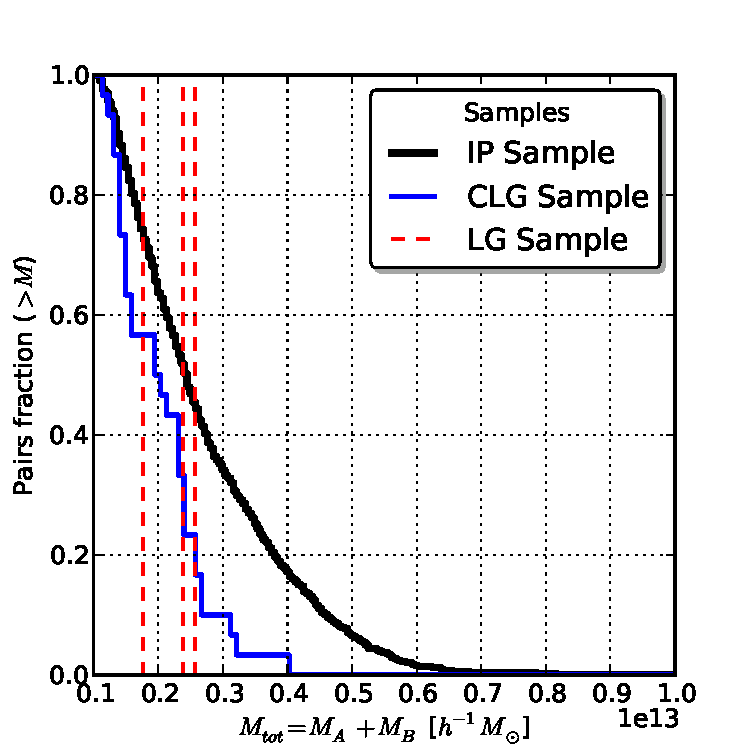
\includegraphics[trim = 0mm 0mm 9.5mm 10mm, clip, width=0.45\textwidth]
	{./figures/4_results/IP_IMF.pdf}
	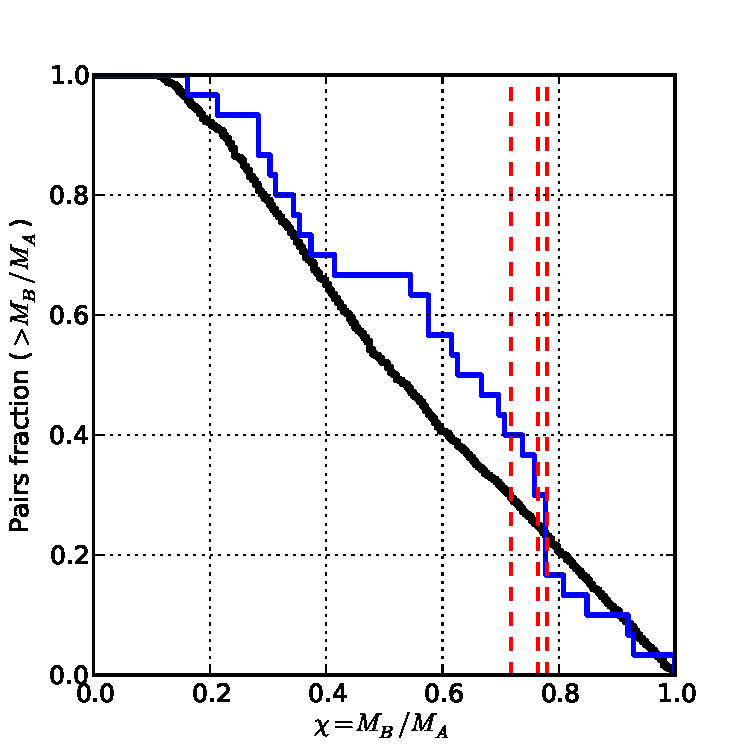
\includegraphics[trim = 0mm 0mm 9.5mm 10mm, clip, width=0.45\textwidth]
	{./figures/4_results/IP_Mass_Ratio.pdf}
	
	\caption{\small{ Integrated histograms for the total mass $M_{A} + 
	M_{B}$ (left panel) and the mass ratio $M_B/M_A$ (right panel), of the
	pair samples in Bolshoi. }}
	\label{fig:CLG_Mass}
\end{figure}
%.........................................................................


%Reviewed
An interesting result of this figure is that the ranges associated to the
\textit{LG} sample in CLUES are well-defined (vertical red lines). This 
evidence that \textit{LG} systems share not only a same cosmological 
environment but a similar distribution of mass. As a possible explanation 
to this, it can be considered a selection effect in the samples due to the
construction of the constrained simulations, while a more optimist point 
of view would be considering this as an evidence of a correlation between
the mass and the local environment of the pair.


%Reviewed
In order to answer the last question, it must be analysed the distribution
of both mass parameter for the other samples. In the case of the total 
mass for \textit{IP} systems, it is distributed according to the same 
distribution of halos (see Figure \ref{fig:IMF}), as it is expected due
to there is no restrictions regarding the environment. In the case of
the mass ratio, it is obtained a distribution completely homogeneous. Now,
for the \textit{CLG} sample, which it is expected to be influenced by the 
environment, it is obtained a biased distribution of the total mass 
regarding the \textit{IP} sample and centred approximately in the range
defined by the \textit{LG} systems. For the distribution of mass ratios
of \textit{CLG} systems, it is also found a uniform behaviour due to the
lack of data, in spite of that, there is an apparent over-abundance around
the mean value defined by the \textit{LG} systems, but again, there are 
no data enough in order to conclude a possible relation.


%Reviewed
\newpage
%.........................................................................
%Dispersion diagram for pairs mass parameters
\begin{figure}[htbp]
	\centering
	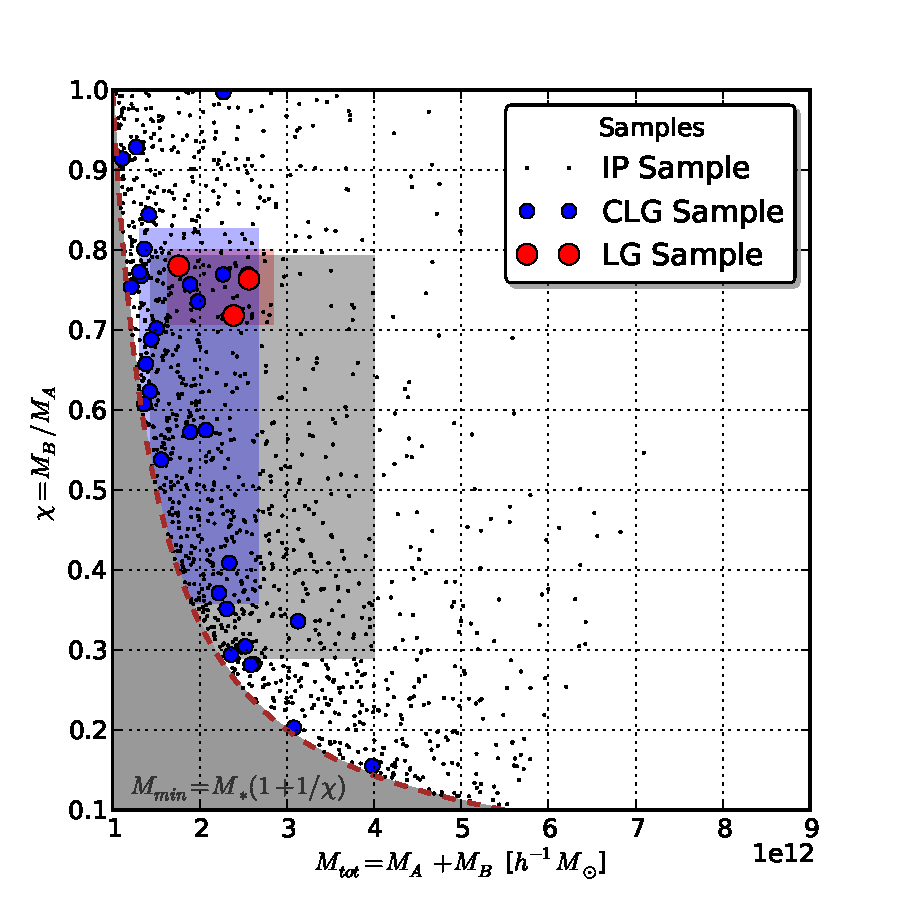
\includegraphics[trim = 0mm 0mm 0mm 10mm, clip, width=0.8\textwidth]
	{./figures/4_results/IP_Mass_vs_Ratio.pdf}
	
	\caption{\small{Diagram of dispersion for the defined mass parameters
	($M_{tot}$,$\chi$) and for each one of the pair samples. The 
	square regions are made from the mean value and the standard deviation
	of the respective sample (same colour). The gray regions in the bottom
	corresponds to a cut off artificially imposed due to the minim mass 
	range of the halos ($M_*$) for constructing the pair samples.}}
	\label{fig:Dispersion_Mass_CLG}
\end{figure}
%.........................................................................


%Reviewed
In the Figure \ref{fig:Dispersion_Mass_CLG}, it is shown a diagram of 
dispersion for the mass parameters previously defined for the pair samples.
The square regions represent the mean value and one standard deviation 
regarding the parameters labelled in each axis, what allows comparing the
different distributions graphically. From this comparison it is confirmed 
that the proposed method for constructing \textit{CLG} systems biases the 
total mass of pair systems within a range consistent with the mass of 
\textit{LG} systems in the constrained simulations, whereas there is any
selection effect regarding the mass ratio $\chi$.


%Reviewed
Finally, and with the aim of answering if there is a possible effect due
to the local environment on the total mass of \textit{CLG} systems, it is
computed in the next Figure \ref{fig:CLG_FA_Mass} diagrams of correlation
between the fractional anisotropy and the mass parameters.


%Reviewed
\
%.........................................................................
%Correlation Mass-FA
\begin{figure}[htbp]
	\centering
	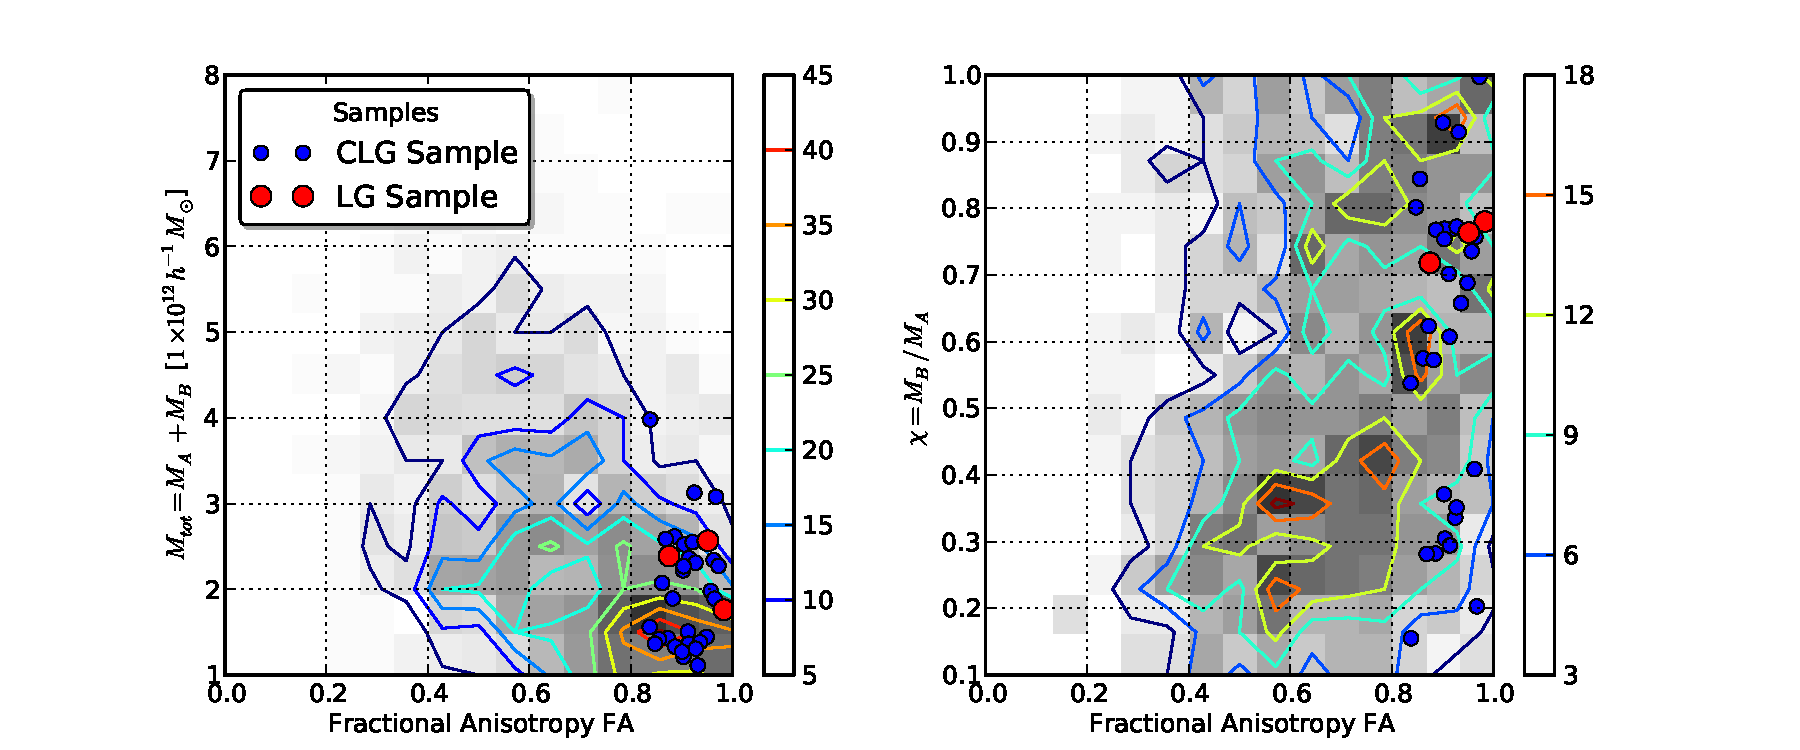
\includegraphics[trim = 25mm 0mm 35mm 10mm, clip, width=1.0\textwidth]
	{./figures/4_results/CLG_FA_Mass.pdf}
	
	\caption{\small{Diagrams of dispersion for the fractional anisotropy
	with respect to the mass parameters. The background map and the contour
	curves correspond to the \textit{IP} sample.}}
	\label{fig:CLG_FA_Mass}
\end{figure}
%.........................................................................
\

%Reviewed
In the case of the total mass $M_{tot}$ of the \textit{IP} samples, it can
be noticed that pairs with low mass values lie preferentially within high
anisotropy regions, while pairs with higher mass values lie within middle
anisotropy regions. This can be thought as a correlation between the local
environment and the total mass for the \textit{IP} sample, whereof it is 
concluded that the criterion of construction of the \textit{CLG} sample
by using the properties of environment of the \textit{LG} systems selects
low mass pairs.


%Reviewed
For the mass ratio $\chi$, it is noticed a more dispersed distribution for
the \textit{IP} sample. In spite of that, it is noticed a slight 
over-abundance of pairs with low $\chi$ values in middle anisotropy 
regions, while in high anisotropy regions there are more pairs with 
higher $\chi$ values. This is consistent with the performed selection in
the \textit{CLG} sample, for which, approximately $66\%$ of the pairs
have mass ratio values such that $\chi>0.5$. From this it can be intuited
a possible correlation between the host environment and the mass ratio 
$\chi$ of the pairs, but due to the high dispersion of the distribution
and the lack of data, it cannot be concluded.


\newpage

	%---------------------------------------------------------------------
	%Angular momentum and energy
	\subsection{Distributions of Energy and Angular Momentum}
	\label{subsec:AngularMomentumAndEnergy}
	%---------------------------------------------------------------------


%Reviewed
The energy and the angular momentum are other interesting physical 
properties of the pair systems. This quantities are defined here from the
next expressions



%.........................................................................
%Energy of Pairs
\eq{eq:EnergyPairs}
{ e_{tot} = \frac{1}{M_A + M_B}\cor{ \frac{1}{2}\pr{ M_A v_A'^2 + M_B v_B'^2 } 
 - G\frac{M_A M_B}{| \bds r_A' - \bds r_B' |}}
 }
%.........................................................................


%Reviewed
%.........................................................................
%Angular Momentum of Pairs
\eq{eq:AMomentumPairs}
{ \bds L_{orb} = \frac{1}{M_A + M_B}\cor{ M_A\bds r_A' \times \bds v_A' + 
M_B\bds r_B' \times \bds v_B' }}
%.........................................................................
where $\bds r_i'$ is the comoving position of the $i$ halo and $\bds v_i'$
is the total velocity\footnote{ Total velocity because it is included the
peculiar term and the Hubble flux with respect to the center of mass of
the systems, so $\bds v_i' = \bds v_{pec,i} + H_0 \bds r_i'$.} with 
respect to the center of mass of the pair.


%Reviewed
%.........................................................................
%Energy-AMomentum Dispersion
\begin{figure}[htbp]
	\centering
	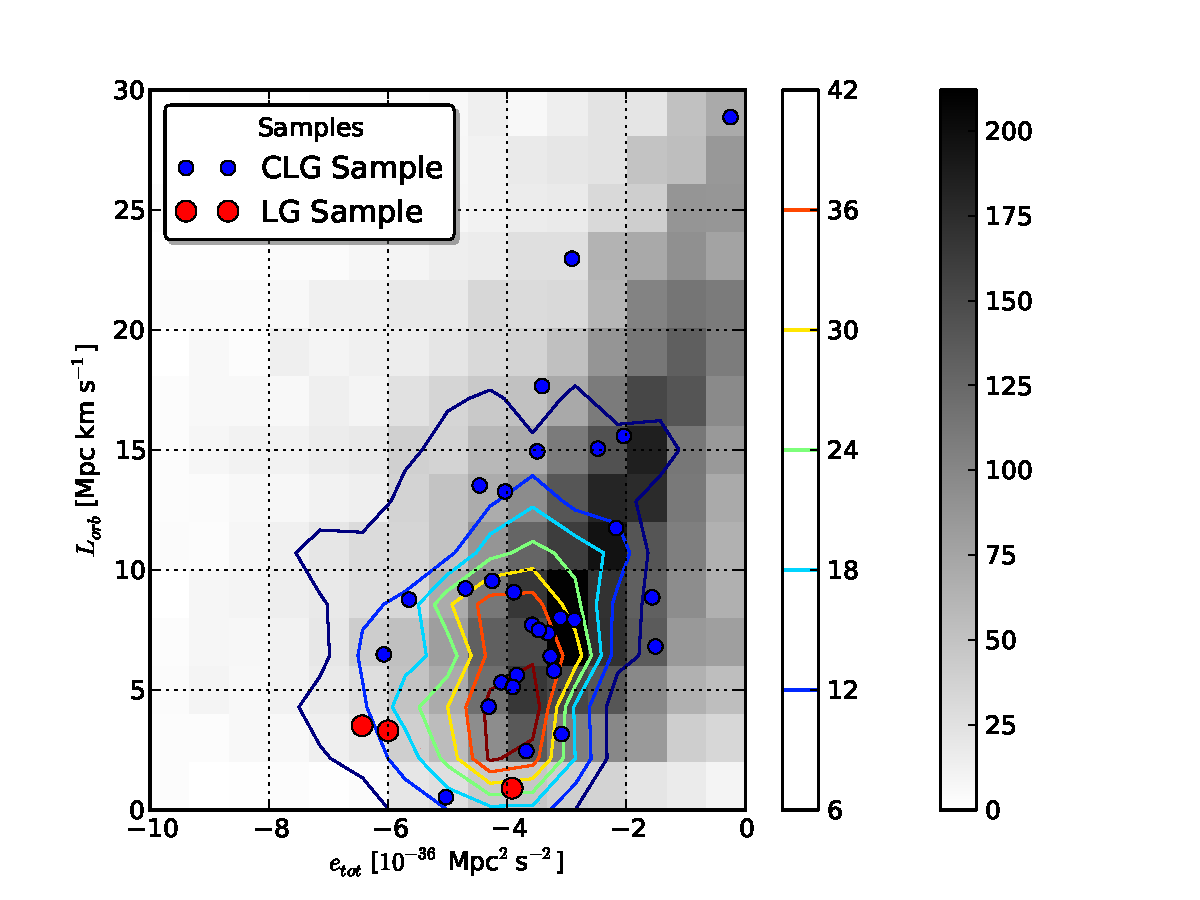
\includegraphics[trim = 8mm 0mm 25mm 10mm, clip, width=0.8\textwidth]
	{./figures/4_results/CLG_E_vs_L.pdf}
	
	\caption{\small{Diagram of dispersion for the total energy and the 
	orbital angular momentum of pair systems. The background map
	corresponds to the distribution of the \textit{P} sample, while the
	contour lines to the distribution of the \textit{IP} sample, in both
	cases the value corresponds to the number of pairs. }}
	\label{fig:CLG_E-L}
\end{figure}
%.........................................................................	


%Reviewed
In the Figure \ref{fig:CLG_E-L} it is shown the distributions of the 
specific total energy and the specific orbital angular momentum for the 
samples. The first result that can be noticed is a significant bias 
between the distribution of the \textit{IP} systems with respect to the 
\textit{P} sample, what demonstrates that the criterion of gravitational 
isolation previously defined in the subsection \ref{subsec:SampleOfPairsToUse}
selects a range of energy and angular momentum lower than the general 
sample of pairs, being the \textit{IP} gravitationally more bounded. In
the case of the \textit{CLG} sample, its distribution is similar to the
\textit{IP} one, whereof there is not an apparent selection due to the
host environment. Finally, it is interesting to notice that the properties
of the three \textit{LG} systems of CLUES are quite similar, thereby 
indicating that they represent a well-defined type of systems, although
as it has been mentioned, this can be a priori effect due to 
the construction of the CLUES simulations.


%Reviewed
\
%.........................................................................
%Correlation Energy, L_orb-FA
\begin{figure}[htbp]
	\centering
	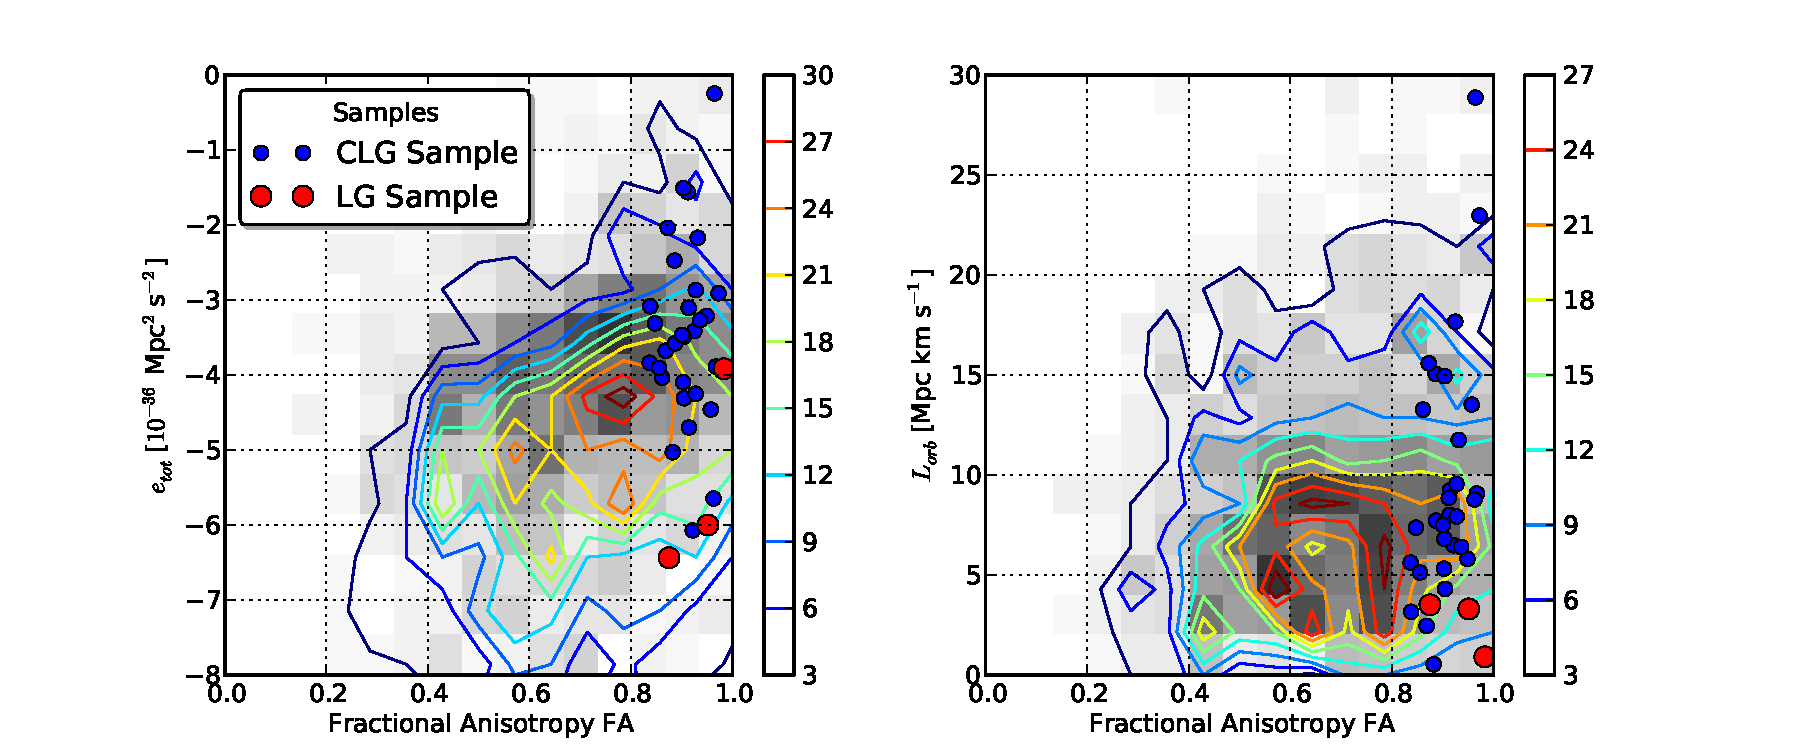
\includegraphics[trim = 20mm 0mm 35mm 10mm, clip, width=1.0\textwidth]
	{./figures/4_results/CLG_FA_E-L.pdf}
	
	\caption{\small{Diagrams of dispersion for the fractional anisotropy 
	with respect to the energy and the angular momentum. The background
	map and the contour curves correspond to the number of pairs of the
	\textit{IP} sample.}}
	\label{fig:CLG_FA_E-L}
\end{figure}
%.........................................................................


%Reviewed
In the Figure \ref{fig:CLG_FA_E-L}, and with the aim of determining 
possible correlations, it is calculated diagrams of correlation for the 
energy and the angular momentum regarding the fractional anisotropy. In 
the case of the specific energy, \textit{IP} pair systems with higher
values of energy (less bounded), seem to be mostly distributed over high
anisotropy regions, whereas low energy systems (more bounded) are 
preferentially within middle anisotropy regions, what shows a correlation
between these two quantities. For \textit{CLG} systems, the selection by
using the environment biases the distribution of energy to higher energy 
values than the mean distribution for \textit{IP} systems, what is 
consistent with the found correlation. In this case, the \textit{LG} 
systems seem to not follow this correlation, having much lower values of 
energy than expected. Finally, for the distribution of specific angular 
momentum, there is no a clear correlation, being any $L_{orb}$ value of
the pairs equally probable for any type of environment.


	
	%---------------------------------------------------------------------
	%Alineación del momentum angular
	\subsection{Angular Momentum Alignment}
	\label{subsec:AngularMomentumAlineation}
	%---------------------------------------------------------------------
	
%Reviewed
Finally, the last property to be analysed  for the pair systems, it is 
their alignment regarding the cosmological environment. For this it is 
defined the angle $\phi_i$ as the angle formed between the eigen-vector 
$\bds u_{\lambda i}$ of the V-web and the angular momentum of the $i$ 
pair system $\bds L_{orb}$.


%Reviewed
%.........................................................................
%CLG Alineation
\begin{figure}[htbp]
	\centering
	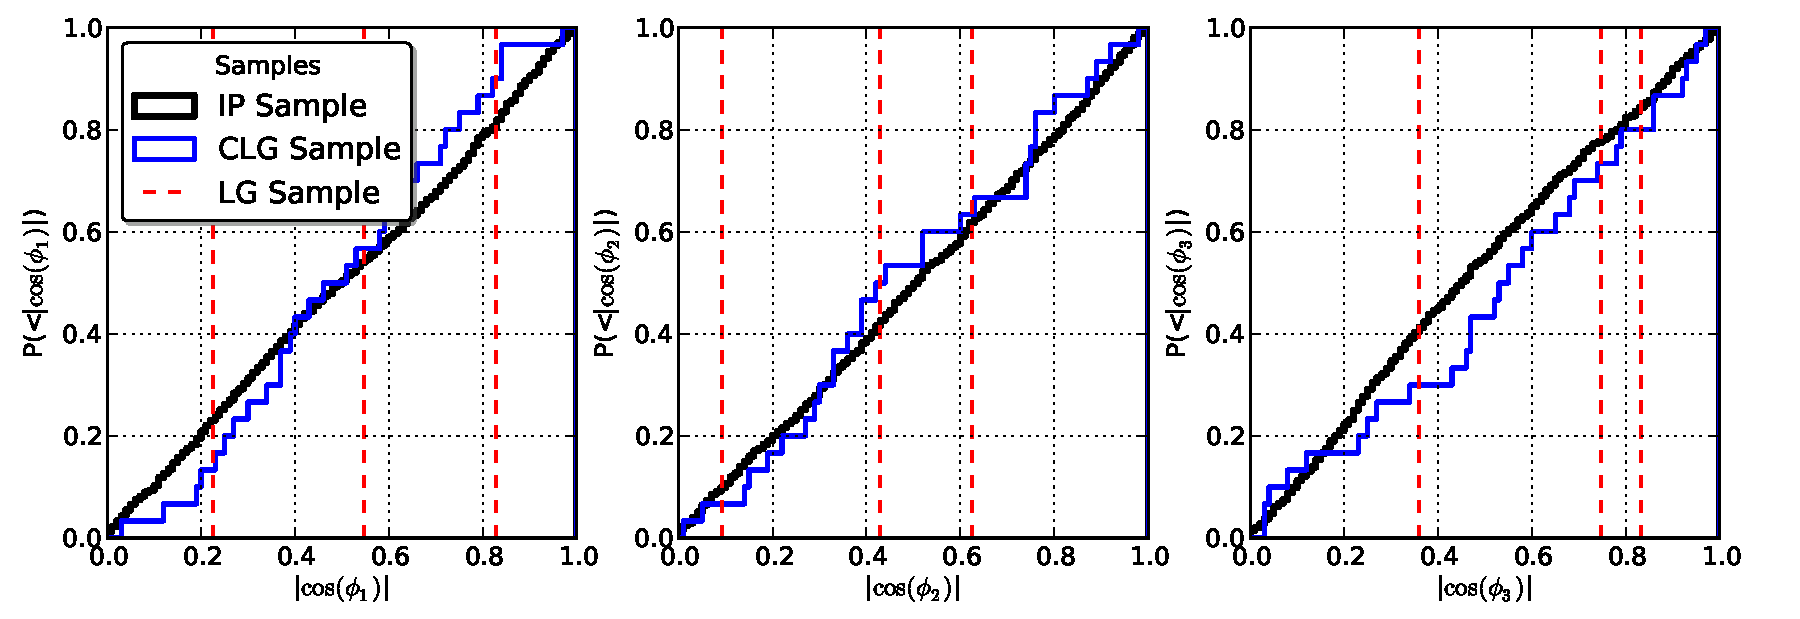
\includegraphics[trim = 0mm 0mm 5mm 0mm, clip, width=1.0\textwidth]
	{./figures/4_results/CLG_Alineation.pdf}
	
	\caption{\small{Integrated histograms for the angle formed between
	the angular momentum of each pair, that determines the orbital plane,
	and each one of the eigen-vectors defined by the V-web regarding the
	cosmological environment. It is performed for each one of the pair 
	samples, \textit{IP} and \textit{CLG}, whereas the \textit{LG}systems 
	in CLUES are plotted with vertical red dashed lines.}}
	\label{fig:CLG_Alineation}
\end{figure}
%.........................................................................
	

%Reviewed
In the Figure \ref{fig:CLG_Alineation}, it is calculated the integrated
histograms for each one of the defined angles $\phi_i$. As it can be 
noticed, the \textit{CLG} and \textit{IP} samples are homogeneous 
regarding the three distributions of angles, thereby indicating that there
is no a preferred alignment with regard to the cosmological environment.
This also is evidenced for the single values of the \textit{LG} systems of
the constrained simulations.



%*************************************************************************



	
%*************************************************************************
%Conclusions
\section{Conclusiones}
\label{sec:Conclusions}


Esta sección está dedicada a compilar los principales resultados obtenidos
en este capítulo. Estos serán enumerados y discutidos acorde al órden en
que fueron obtenidos.


%.........................................................................
%Main Results
\begin{enumerate}
\item[\textbf{1.}] La construcción de la muestra \textit{IP} fue 
inicialmente propuesta en \cite{forero2011} con el objetivo de reproducir
sistemas tipo grupo local. A pesar de esto, el número de estos sistemas 
encontrados en la simulación Bolshoi es mucho mayor al que se espera acorde
a la abundancia de \textit{LG} en simulaciones restringidas. El método 
propuesto para la selección de la muestra \textit{CLG} en Bolshoi a partir 
del entorno cosmológico de los \textit{LG}, produce un número de sistemas 
que concuerda con los encontrados en la simulaciones restringidas, escalando 
apro\-ximadamente como el volumen de las simulaciones. Más aún, aplicando 
este mismo método en las simulaciones restringidas se halla una muestra
con un tamaño similar a la \textit{LG}.


\item[\textbf{2.}] A partir de los valores medios de densidad en las 
diferentes regiones del entorno cosmológico (figura \ref{fig:Vol_Fraction})
se propone un esquema para la elección de un rango óptimo del parámetro
$\lambda_{th}$ de la V-web con el objetivo de reproducir la 
apariencia visual de la red cósmica. Este está basado en la 
minimización de la densidad media en las regiones de vacío debido a que
son las dominan la apariencia del campo de densidad a gran escala. Con
esto se garantiza que las regiones vacías no invadan regiones de más alta
densidad, que en principio deben ser clasificadas como hojas o filamentos.
Este método da un rango de valores óptimos aproximadamente igual para 
todas las simulaciones usadas ($0.2 \leq \lambda_{th} \leq 0.4$), además
reproduce adecuadamente la apariencia visual (ver figura 
\ref{fig:Vweb_Comparison} para $\lambda_{th} = 0.3$). A pesar de esto, 
este parámetro sigue siendo libre y no es viable usar un esquema de 
clasificación basado en este para determinar correlaciones con propiedades
físicas, en vez de esto se introduce el fraccional de anisotropía 
con la normalización usada en \cite{libeskind2013}.


\item[\textbf{3.}] La distribución del entorno cosmológico de las 
simulaciones Bolshoi y CLUES difieren, existiendo un cambio de densidad 
media muy pronunciado entre regiones de vacío y filamentos en Bolshoi, 
mientras que es mucho más suave en las CLUES. A pesar de esto, las 
fracciones de volumen asociadas a cada tipo de entorno son aproximadamente 
iguales para ambas simulaciones en el rango óptimo determinado para 
$\lambda_{th}$. A pesar de esto, se espera que la dinámica local 
caracterizada por la V-web sea independiente de la estructura global 
de la distribución de entorno, lo cual valida el esquema de selección 
de la muestras \textit{CLG} en Bolshoi.


\item[\textbf{4.}] El método de construcción de los 
\textit{CLG} selecciona un entorno cosmológico común para estos 
sistemas, siendo preferidas zonas de vacío y hojas no muy planas.
Estas regiones presentan una alta anisotropía, cuantificada por el 
fraccional de anisotropía FA. En el caso de los sistemas \textit{IP},
estos se encuentran en zonas de media a alta anisotropía, asociadas 
a valores de baja densidad, contrario a los halos que están en zonas 
más densas y menos anisotrópicas como filamentos y nudos, aún así 
la distribución de entorno de los \textit{IP} es amplia y no pueden
ser asociados a un tipo de entorno específico. El sesgo producido
entre los \textit{IP} y los halos generales se debe al criterio
de aislamiento gravitacional usado para construir los \textit{IP},
esto hace que zonas con mayor densidad de halos sean menos aptas por
la alta influencia gravitacional.


\item[\textbf{5.}] Se encuentra una correlación entre la masa total de 
los pares de la muestra \textit{IP} y el fraccional de anisotropía del 
entorno, donde masas mayores son más abundantes en regiones de 
anisotropía media mientras masas menores se presentan con mayor 
frecuencia en zonas de alta anisotropía. Esto implica que la selección
de entorno realizada en los \textit{CLG} reproduce un rango de masa menor.
En el caso de la razón de masa, no se encuentra ninguna correlación 
significativa con el entorno, aún así se nota una ligera sobreabundancia 
de razones de masa mayores en regiones más anisotrópicas, pero es 
necesaria más estadística para poder ser algo concluyente.


\item[\textbf{6.}] Se halla un correlación para la energía específica
de los sistemas \textit{IP} respecto al entorno, obtiendo valores más
altos en regiones más anisotrópicas y valores bajos en regiones de 
anisotropía media. Esta correlación parece seleccionar un rango de 
energía para los sistemas \textit{CLG}, aunque esta no es consistente
con los valores obtenidos de los \textit{LG}. Para el momentum angular
no se encuentra ninguna correlación con el entorno.


\item[\textbf{7.}] Finalmente se encuentra que no existen alineaciones
privilegiadas entre el momentun angular de los pares \textit{CLG} (o de 
su plano orbital) y las direcciones de los autovectores de la V-web.


\end{enumerate}
%.........................................................................


%*************************************************************************